\section{Correction Principles}


% ===============================
%        Response Matrix
% ===============================
\subsection{\review{Response Matrix}}

A response matrix is a linear equation system that describes the change of an observable for a set of individual multipole strengths. By taking the pseudo-inverse of this matrix and multiplying it to the measured observables, a set of corrector strengths if obtained that can replicate the measured value. Taking the opposite sign then gives a correction.
This technique is routinely used to correct, amongst others, \beta-beating as well as Resonance Driving Terms. In situations where measurements are taken at each BPM for a particular observable, the corresponding response matrix ends up containing over 500 values per corrector, for a single beam.

Individual MAD-X simulations are run with a single multipole powered at a time. The resulting parameter values (e.g. \beta-beating) are then compared to those obtained from a simulation without any powering, allowing to determine the specific impact of each multipole.

A response matrix is thus created following eq.\ref{eq:resp_matrix}, for a matrix of observables $O$, a reference matrix of observables without any corrector $O_R$ and a fixed multipole strength $k$. Given measured data $M$, the set of correctors needed to compensate the values can be obtained by taking the pseudo-inverse of the matrix in eq.\ref{eq:resp_matrix_inverted}.

\begin{equation}
  R = \left(O - O_R \right) \cdot \frac{1}{k}
  \label{eq:resp_matrix}
\end{equation}

\begin{equation}
  \begin{bmatrix}
    k_1 \\
    \vdots \\
    k_n \\
  \end{bmatrix}
  = -(R^{+} \cdot M)
  \label{eq:resp_matrix_inverted}
\end{equation}
 
Response matrices are very versatile and can combine several observables to be corrected by the same multipoles. One example, detailed later in this thesis, is the third order chromaticity and the resonance driving term $f_{1004}$, both contributed to by decapoles.

\subsubsection{Example}

In this example, simulations are run with MAD-X PTC to correct the third chromaticity in the LHC.
$Q'''$ is taken from \verb|ptc_normal| for each beam and axis, with \verb|MCDs|, decapole correctors, powered with a fixed strength one at a time. A scaling factor is applied to get the change of chromaticity for one unit of $K_5$.
8 correctors are used, which strengths are denoted $k_1$ through $k_8$.
Transposes are only used to make the equations easier to display.\\
The values in Tab.\ref{table:resp_matrix_example} are corrected via 
Eq.~\eqref{eq:resp_matrix_inverse_example} after having built the response matrix in Eq.~\eqref{eq:resp_matrix_example}.

\begin{table}[H]
  \center
  \begin{tabular}{c c c}
      Observable & Value \\
      \hline
      $Q'''_x$ & -666111 \\
      $Q'''_y$ &  121557 \\
  \end{tabular}
  \caption{Example chromaticity values to correct via a response matrix}
  \label{table:resp_matrix_example}
\end{table}

% ====
\vspace{0.4cm}
\begin{equation}
  R
  %
  =
  %
  \left(
    %{\text{Individual} \atop \text{simulations}}
    {\genfrac{}{}{0pt}{0}{\text{Individual}}{\text{simulations}}}
    \left\{
      \begin{bNiceMatrix}
       -155899  &  122004 \\  
       -254584  &  138368 \\
       -122715  &  106709 \\
       -218597  &  110686 \\
       -134140  &  106463 \\
       -245791  &  118951 \\
       -147035  &  116544 \\
       -219537  &  112317 \\
        \CodeAfter
        \OverBrace{1-1}{1-1}{Q'''_x}[yshift=2mm]
        \OverBrace{1-2}{1-2}{Q'''_y}[yshift=2mm]
      \end{bNiceMatrix}^T
    \right.
    -
    \left.
    \begin{bNiceMatrix}
       5135 \\
       8470 \\
      \CodeAfter
      \OverBrace{1-1}{1-1}{\scriptstyle \text{Reference}}[yshift=2mm]
    \end{bNiceMatrix}
    \right\}
    {\genfrac{}{}{0pt}{0}{Q'''_x}{Q'''_y}}
  \right)
  %
  \cdot
  %
  \underbrace{\frac{1}{-1000}}_{\text{Corrector strength}}
  \label{eq:resp_matrix_example}
\end{equation}
\vspace{0.5cm}


% Inverting the response matrix
\begin{equation}
    \begin{matrix}
      k_1 \\
      k_2 \\
      k_3 \\
      k_4 \\
      k_5 \\
      k_6 \\
      k_7 \\
      k_8 \\
    \end{matrix}
  \left\{
  \begin{pmatrix}
     -1235 \\
      1032   \\  
     -1394  \\ 
      1449   \\ 
     -1043  \\ 
      1864   \\ 
     -1187  \\ 
      1369   \\ 
  \end{pmatrix}
  \right.
  %
  =
  %
  -R^{+} 
  %
  \cdot
  %
  \left.
  \begin{pNiceMatrix}
      -666111 \\
      121557 \\
  \end{pNiceMatrix}
  \right\}
  %{\text{Measured} \atop \text{values}}
  {\genfrac{}{}{0pt}{0}{\text{Measured}}{\text{values}}}
  \label{eq:resp_matrix_inverse_example}
\end{equation}





% ===============================
%    Chromaticity Global Trim
% ===============================
\subsection{\review{Global Trims for Chromaticity}}

% ~~~~~~~~~~~~~~~~~~~~~~~~~~~~~
% The script for the linearity can be found in
% /afs/cern.ch/work/m/mlegarr2/public/jupyter/chromaticity/simulations/linearity_dq3_mcd

As per the placement of the MCO and MCD spool piece correctors in the LHC 
layout~\cite{maclean_commissioning_2016-1}, $\beta$-functions at their location are slightly
different from arc to arc. This slight imbalance leads theoretically to the possibility of
correcting the horizontal and vertical axes of the second and third order chromaticity
independently, via a response matrix approach. In practice, the required strength to do so would
exceed those of the design of the correctors.

Another way to correct the chromaticity is via a global uniform trim, where every available
corrector is powered to the same strength.  Simulations are run with \verb|ptc_normal| via MADX-PTC
to obtain the response in chromaticity for a given strength. Chromaticity being linear with
multipole strength, an affine function can be determined for each axis. Figure
\ref{fig:corrections-dq3_versus_k5} shows a simulation with several MCD strengths, highlighting this
linear relation between $Q'''$ and $K_5$, while
Equation~\eqref{eq:corrections:chromaticity_affine_function_ptc} shows an example of such functions computed
at injection energy for the 2022 optics.

\begin{figure}[H]
  \centering
  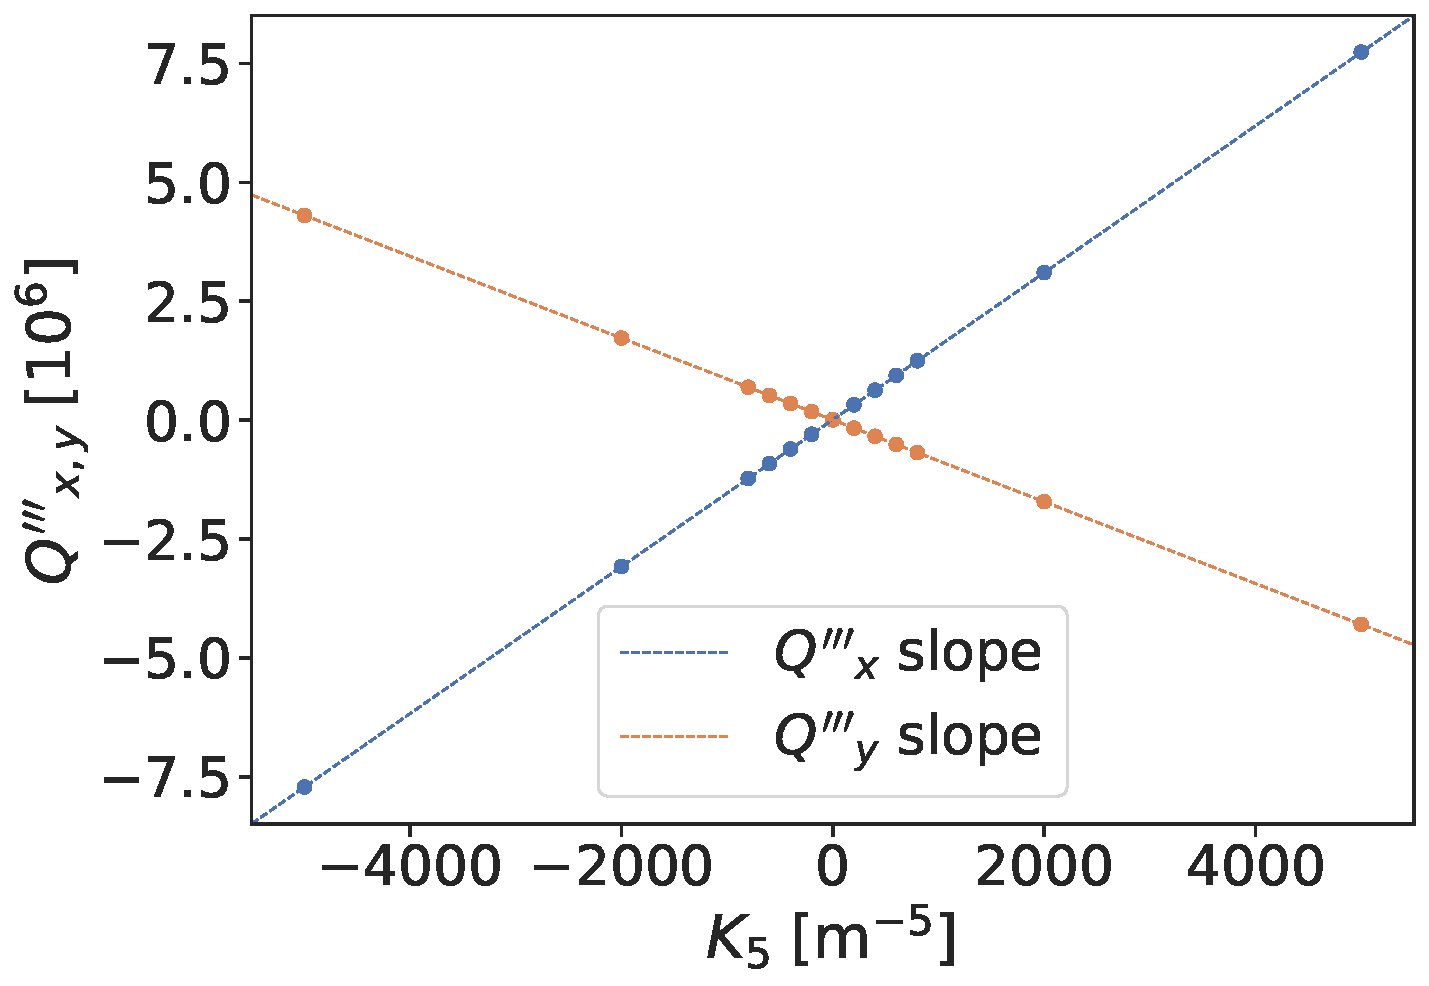
\includegraphics[width=0.6\textwidth]{images/dq3_k5.pdf}
  \caption{Linear relation between the third order chromaticity and decapole corrector strengths,
           simulated with MADX-PTC.}
  \label{fig:corrections-dq3_versus_k5}
\end{figure}

\begin{equation}
  \begin{aligned}
    &Q'''_x = 1533 \cdot \Delta K_5 + 6680 \\
    &Q'''_y = -860 \cdot \Delta K_5 + 5647
  \end{aligned}
  \label{eq:corrections:chromaticity_affine_function_ptc}
\end{equation}

Only the linear part is relevant, as the offset is generated by other multipoles and field errors.
It is thus constant for a configuration where only the relevant spool pieces are used.

Corrections involve minimizing both axes, typically where $Q'''_x$ meets $Q'''_y$:

\begin{equation}
  \Delta K_5 = -\frac{(Q'''_x - Q'''_y)}{\text{slope}_{Q'''_x} - \text{slope}_{Q'''_y}}
  \label{eq:corrections:chromaticity_global_correction}
\end{equation}